\subsection{Ansteuerung Motor Ballnachschub}
\label{sec:dc}
Die Ansteuerung für den Motor für den Ballnachschub wird in in der Gruppe 
PREN-ET entwickelt. (Siehe \ref{sec:pren-et} \nameref{sec:pren-et})
%Daher werden hier nur Anpassungen für das Team 27 betrachtet. 
\begin{figure}[h!]
    \centering
    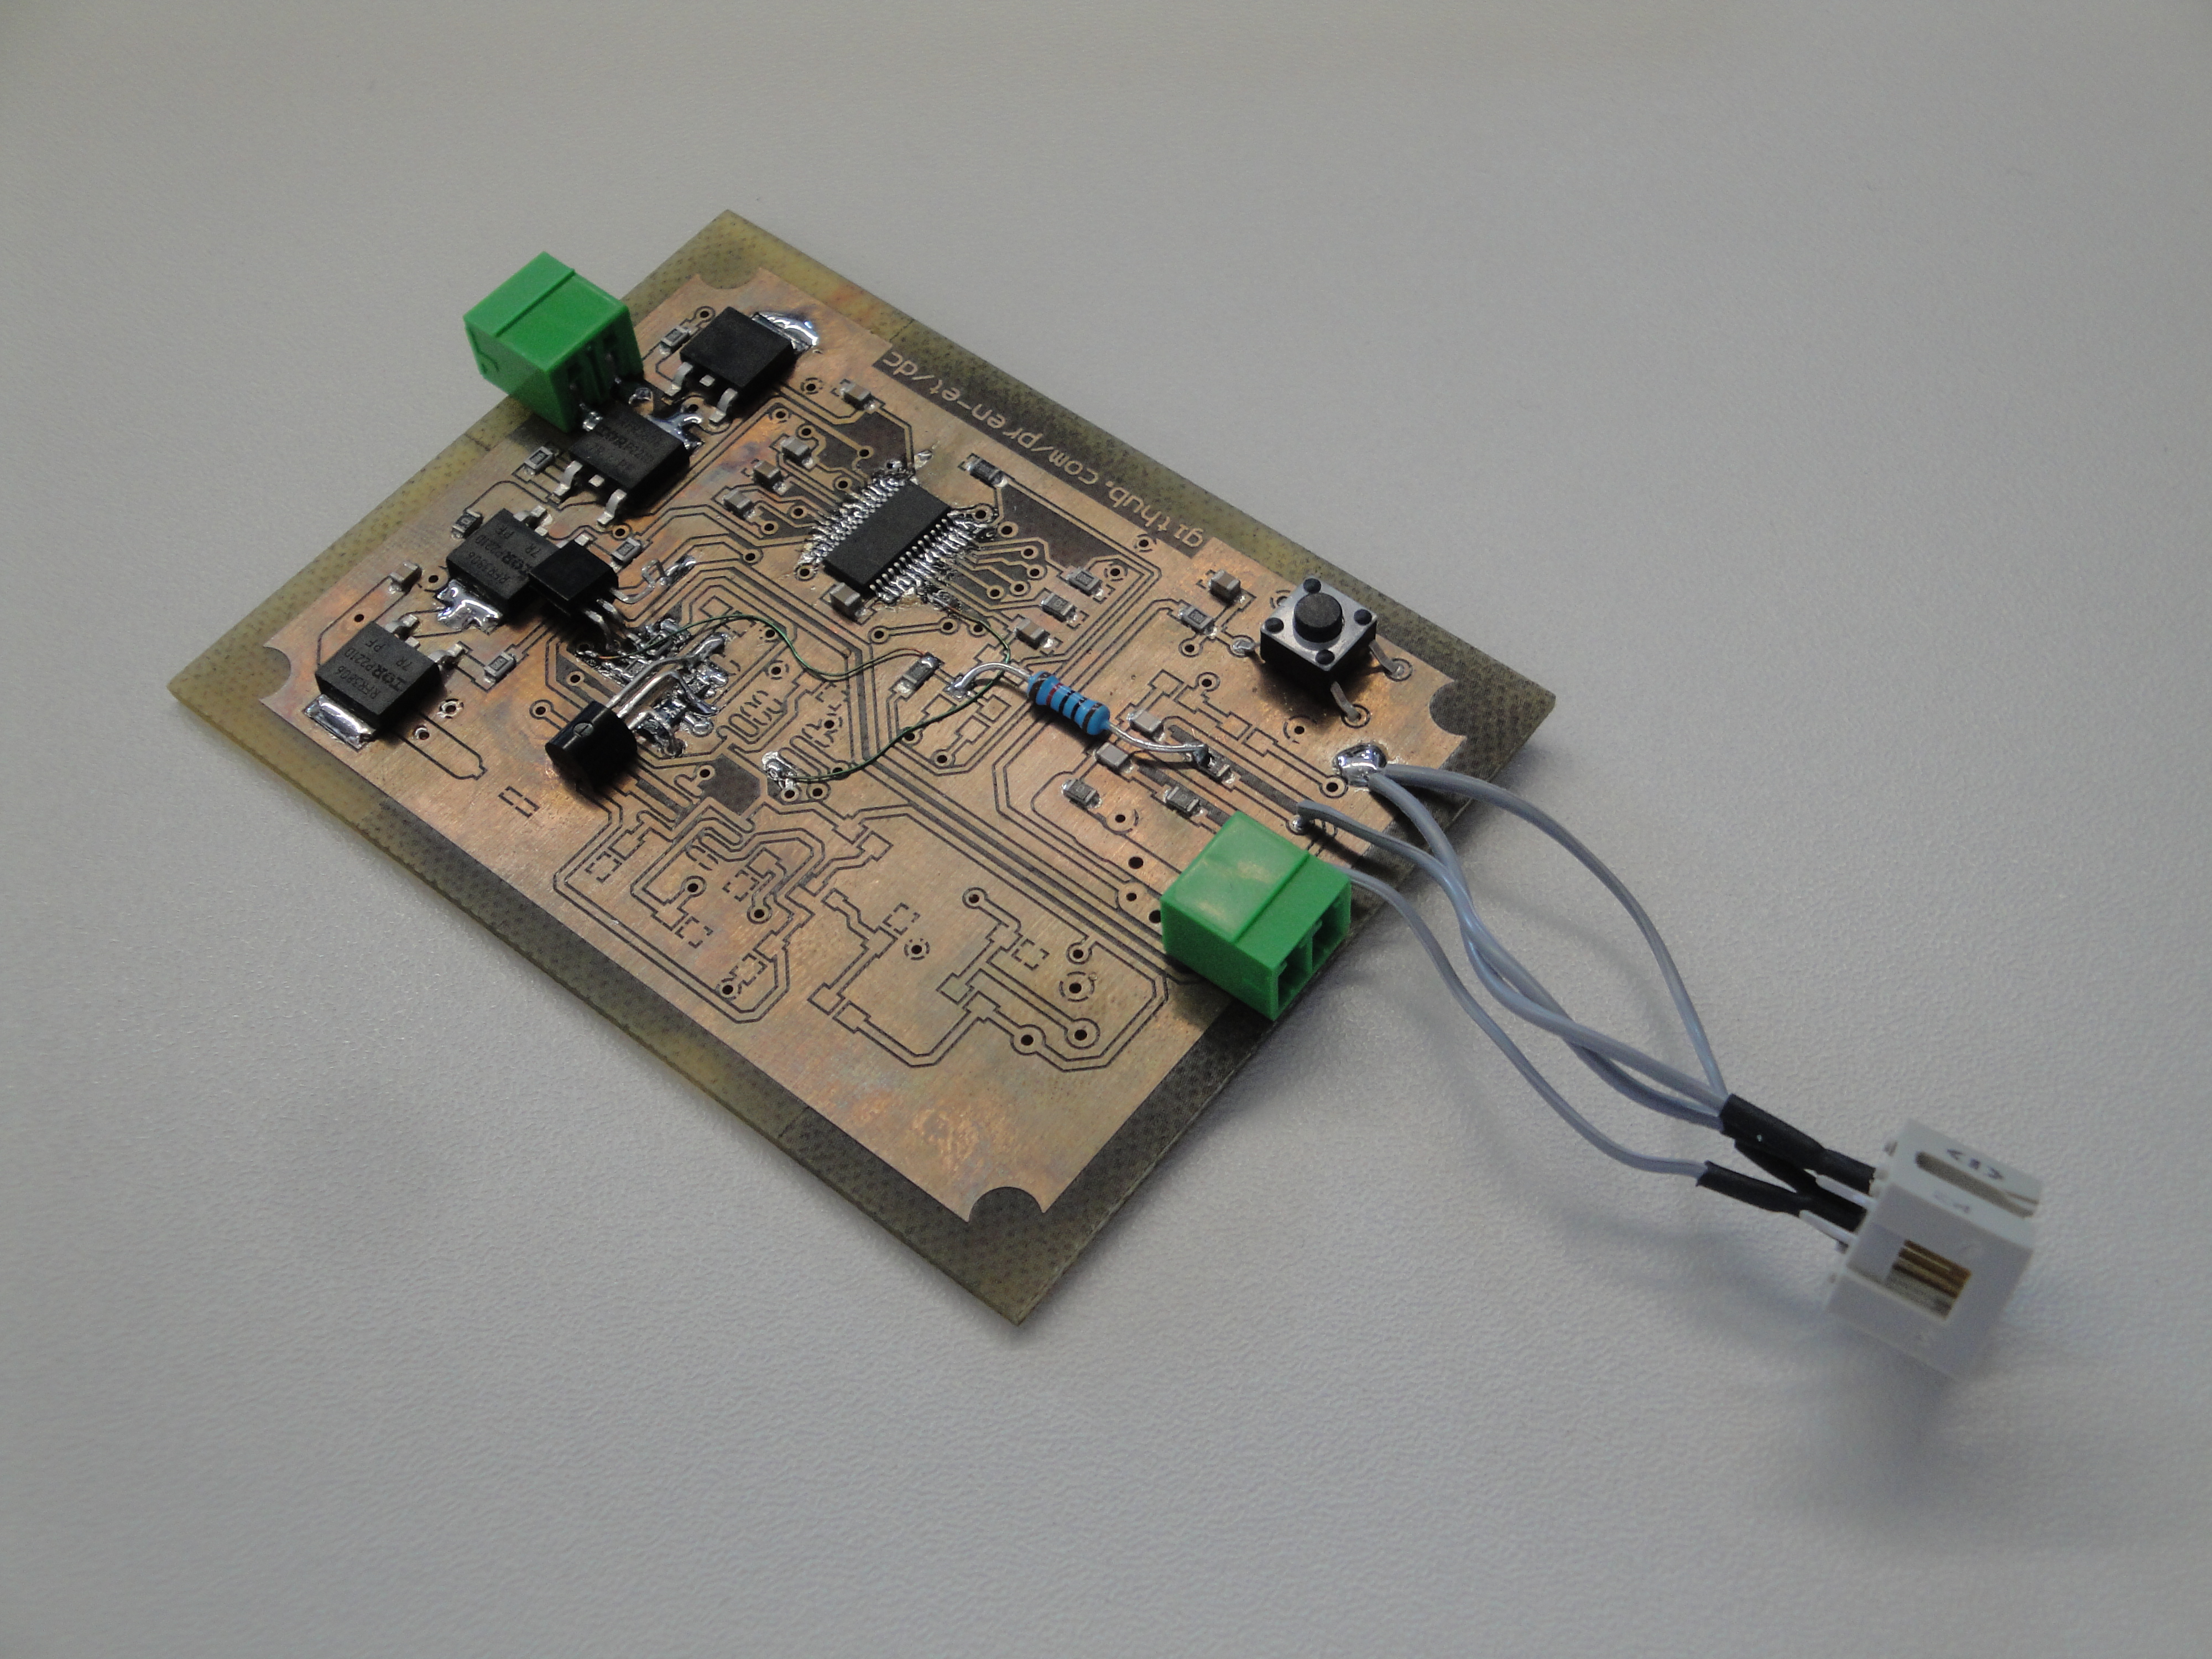
\includegraphics[width=0.7\textwidth]{fig_pcb/DSC02909.JPG}
    \caption{Ansteuerung Ballnachschub}
    \label{fig:dc}
\end{figure}

\noindent
Der Gleichstrommotor für den Ballnachschub wird mit einem 
PWM\footnote{\textbf{P}ulse \textbf{W}idth \textbf{M}odulation} Signal 
angesteuert. Über das Puls-Pausen-Verhältnis kann die Leistung des Motors 
eingestellt werden. 
